\section{Mapping Ground View to Map Location}
The problem solved in this section can be described as follows:
\newline
Given the continuously alternating position of a man walking around in a
ground-view image sequence, find and display his position in a top-view map.

More generally:
\newline
Given a position in a planar projection of a space, find and display the
corresponding position in another planar projection of the same space.

\begin{figure}[ht]
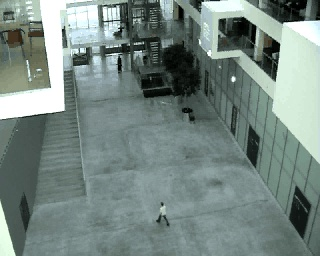
\includegraphics{./pics/Ground.jpg}
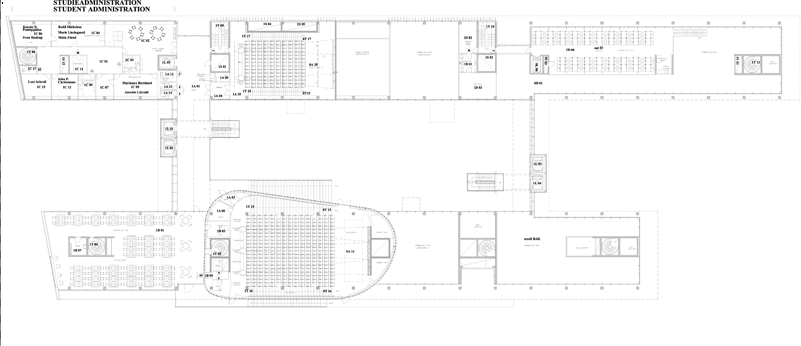
\includegraphics{./pics/ITUMap.png}
\caption{Top: Ground-view. Bottom: Top-view map}
\label{fig:groundvsmap}
\end{figure}

The ground-view image and top-view map are seen in figure
\ref{fig:groundvsmap}. Because they are planar projections of the same space, there
exists a homography between the ground floor in the ground-view image ($G$) and the ground floor in the top-view map ($M$). To find this
homography, a user manually selects four corresponding points on the ground
floor in each image, which are then inserted in a system of linear equations. The solution
to which is the homography $H_{G}^{M}$.
Because the camera is static, the same homography can be used in all frames.
Had the camera moved, the ground floor would no longer be projected to the
plane $G$ in the image, and a new homography would be needed.

For each frame in the video sequence, the point $x$ in $G$ is premultiplied
with $H_{G}^{M}$. The normalized result is the point $x'$ in $M$, that
corresponds to the mans location. $$normalize(H_{G}^{M}*x) = x'$$ The point
representing the mans location in $G$ is chosen as close to his feet as possible.
This is important because the man is \emph{not} in plane $G$, he is
perpendicular to it. Which means $H_{G}^{M}$ could transform his head's
location to a point several meters from his feet's.
On a related note, when the man walks up the stairs, he is moving onto another
plane (or rather planes, as each step is its own plane). Therefore, the
homography used to project the ground floor cannot be used for the stairs.
Because of the camera positioning in the ground-view sequence however, the
stair planes and $G$ are so similar you would have to look closely to see the
error.

